\documentclass{article}

\usepackage{graphicx} 
\usepackage[left=2.5cm, right=2.5cm, top=2cm, bottom=2cm]{geometry}
\usepackage{titlesec}
\usepackage{amsmath}
\usepackage{algorithm}
\usepackage{algpseudocode}
\usepackage{tikz}
\usepackage{caption}
\usepackage{listings}
\usepackage{xcolor}
\usepackage{fancyhdr}
\pagestyle{fancy}
\fancyhf{} % 清空页眉和页脚
\fancyfoot[C]{\thepage} % 只在页脚中居中显示页码
\renewcommand{\headrulewidth}{0pt} % 去掉页眉的横线
\usepackage{tikz}
\usetikzlibrary{trees}
\usepackage{lmodern} % 加載字體
\usepackage[UTF8]{ctex} % 如果你使用的是 macOS 系统
\usepackage{xeCJK}
    \setCJKmainfont[AutoFakeBold=3]{TW-Sung}
    \XeTeXlinebreaklocale "zh"             
    \XeTeXlinebreakskip = 0pt plus 1pt
\usepackage{multirow}
\ctexset{
    figurename = {Figure},  % 設定圖標標題為「圖」
    tablename = {Table}    % 設定表標標題為「表」
}


\titleformat{\section}[hang]{\normalfont\Large\bfseries}{\thesection}{1em}{} 
\titleformat{\subsection}[hang]{\normalfont\bfseries}{\hspace{1em}\thesubsection}{1em}{}
\titlespacing*{\subsection}{2em}{3.25ex plus 1ex minus .2ex}{1.5ex plus .2ex}

\lstset{
    language=Python,
    basicstyle=\ttfamily\small,
    keywordstyle=\color{blue},
    commentstyle=\color{green},
    stringstyle=\color{red},
    showstringspaces=false,
    numbers=left,
    numberstyle=\tiny\color{gray},
    stepnumber=1,
    numbersep=5pt,
    backgroundcolor=\color{white},
    frame=single,
    rulecolor=\color{black},
    captionpos=b
}

\title{Database Management\\Homework 1}
\author{B11705044 \\ Yen-Hung, Chiang}
\date{}

\begin{document}

\maketitle

\section*{1}
\subsection*{(a)}
\begin{table}[h!]
\centering
\begin{tabular}{|c|c|c|c|c|c|}
\hline
Weathersit & Days & Mean(temp) & Median(temp) & Std(temp) & Mean(cnt) \\ \hline
1 & 463 & 20.97 & 21.39 & 7.84 & 4876.79 \\ \hline
2 & 247 & 19.29 & 18.79 & 6.85 & 4035.86 \\ \hline
3 & 21 & 17.77 & 18.04 & 5.39 & 1803.29 \\ \hline
\end{tabular}
\caption{各組別的統計量}
\label{tab:example}
\end{table}
\begin{lstlisting}[caption={(a)小題的 Python Code}]
import pandas as pd
import openpyxl

df = pd.read_excel('Bike.xlsx', engine='openpyxl')
group1 = df.groupby('weathersit')

group1_size = group1.size()
group1_mean = group1['temp'].mean().round(2)
group1_median = group1['temp'].median().round(2)
group1_std = group1['temp'].std().round(2)
group1_mean_cnt = group1['cnt'].mean().round(2)

summary_df1 = pd.DataFrame({
    'Size': group1_size,
    'Mean Temperature': group1_mean,
    'Median Temperature': group1_median,
    'Standard Deviation Temperature': group1_std,
    'Mean Count': group1_mean_cnt
}).reset_index()

print(summary_df1)
\end{lstlisting}

\subsection*{(b)}
\begin{table}[h!]
\centering
\begin{tabular}{|c|c|c|c|c|c|c|}
\hline
Weathersit & Workday & Days & Mean(temp) & Median(temp) & Std(temp) & Mean(cnt) \\ \hline
\multirow{2}{*}{1} & 0 & 156 & 20.19 & 20.10 & 8.01 & 4587.27 \\ \cline{2-7}
\cline{2-7}
 & 1 & 307 & 21.37 & 21.94 & 7.73 & 5023.90 \\ \hline
\multirow{2}{*}{2} & 0 & 70 & 18.99 & 17.72 & 6.93 & 3936.83 \\ \cline{2-7}
\cline{2-7}
 & 1 & 177 & 19.40 & 19.03 & 6.84 & 4075.03 \\ \hline
\multirow{2}{*}{3} & 0 & 5 & 15.59 & 16.26 & 6.14 & 1815.40 \\ \cline{2-7}
\cline{2-7}
 & 1 & 16 & 18.45 & 18.54 & 5.16 & 1799.50 \\ \hline
\end{tabular}
\caption{各組別的統計量}
\label{tab:example}
\end{table}
\begin{lstlisting}[caption={(b)小題的 Python Code}]
import pandas as pd
import openpyxl

df = pd.read_excel('Bike.xlsx', engine='openpyxl')
group2 = df.groupby(['weathersit', 'workday'])

group2_size = group2.size()
group2_mean = group2['temp'].mean().round(2)
group2_median = group2['temp'].median().round(2)
group2_std = group2['temp'].std().round(2)
group2_mean_cnt = group2['cnt'].mean().round(2)

summary_df2 = pd.DataFrame({
    'Size':group2_size,
    'Mean Temperature': group2_mean,
    'Median Temperature': group2_median,
    'Standard Deviation Temperature': group2_std,
    'Mean Count': group2_mean_cnt
}).reset_index()

print(summary_df2)
\end{lstlisting}

\subsection*{(c)}
\begin{table}[h!]
\centering
\begin{tabular}{|c|c|}
\hline
Weathersit & corr. coef.  \\ \hline
1 & 0.622190  \\ \hline
2 & 0.644899  \\ \hline
3 & 0.606836  \\ \hline
\end{tabular}
\caption{三組資料各組內的 temp 和 cnt 的相關係數}
\label{tab:example}
\end{table}
\begin{lstlisting}[caption={(c)小題的 Python Code}]
def compute_corr(group):
    if len(group) > 1:  
        return group[['temp', 'cnt']].corr().iloc[0, 1]
    else:
        return float('nan') 

corr_df = group1.apply(compute_corr).reset_index(name='Correlation')

print(corr_df)
\end{lstlisting}
\begin{figure}[h!]
    \centering
    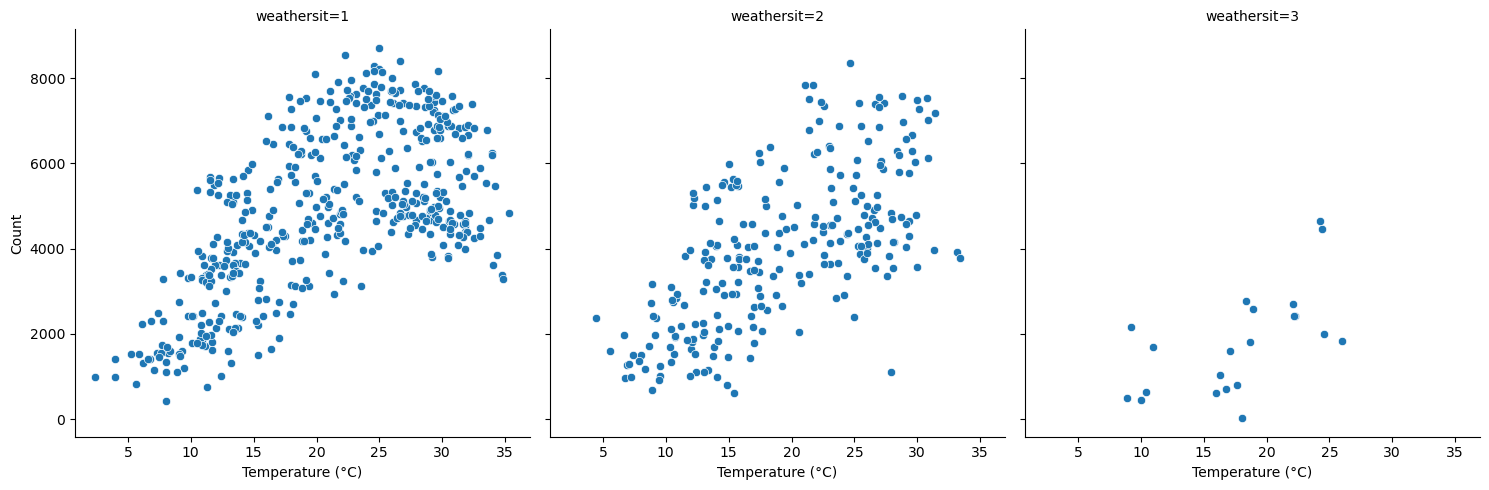
\includegraphics[width=0.8\textwidth]{plot.png}
    \caption{各組資料 temp 和 cnt 的散佈圖。}
\end{figure}
\begin{lstlisting}[caption={產生散佈圖的 Python Code}]
import seaborn as sns
import matplotlib.pyplot as plt

g = sns.FacetGrid(df, col='weathersit', col_wrap=3, height=5)
g.map_dataframe(sns.scatterplot, x='temp', y='cnt')

g.set_axis_labels('temp', 'cnt')
g.set_titles(col_template='weathersit={col_name}')
plt.show()
\end{lstlisting}

\section*{2}
\subsection*{(a)}
\begin{quote}
Assume there is a member function called \texttt{size()} in \texttt{class LinkedList}. It returns the size of the \texttt{LinkedList}.

\begin{itemize}
    \item \texttt{constructor}: Set \texttt{LinkedList} to \texttt{nullptr}.
    
    \item \texttt{enqueue()}: Use \texttt{insert()} to add a node at the bottom of the list.
    
    \item \texttt{dequeue()}: Before dequeuing, check if the queue is empty. 
    \begin{itemize}
        \item If \texttt{isEmpty()} returns \texttt{True}, do nothing.
        \item If \texttt{isEmpty()} returns \texttt{False}, use \texttt{delete()} to remove the node at the front of the list.
    \end{itemize}
    
    \item \texttt{isEmpty()}: If \texttt{size()} is 0, then \texttt{isEmpty()} returns \texttt{True}. Otherwise, it returns \texttt{False}.
    
    \item \texttt{getQueueLength()}: Return \texttt{size()}.
\end{itemize}
\end{quote}

\subsection*{(b)}
\begin{center}
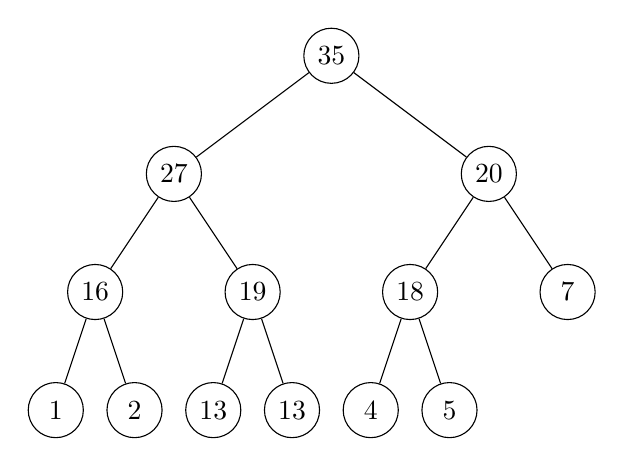
\begin{tikzpicture}[
  level 1/.style={sibling distance=40mm},
  level 2/.style={sibling distance=20mm},
  level 3/.style={sibling distance=10mm},
  edge from parent/.style={draw, -},
  every node/.style={draw, circle, minimum size=7mm, inner sep=1mm}
  ]

  \node {35}
    child {node {27}
      child {node {16}
        child {node {1}}
        child {node {2}}
      }
      child {node {19}
        child {node {13}}
        child {node {13}}
      }
    }
    child {node {20}
      child {node {18}
        child {node {4}}
        child {node {5}}
      }
      child {node {7}}
    };
\end{tikzpicture}
\end{center}

\subsection*{(c)}
\begin{quote}
\begin{minipage}{\textwidth}
\textbf{Root Node:} \\
Store the root node at index 0 in an array.\\[10pt]

\textbf{Leaf Nodes:} \\
Suppose a node stored at index \( i \) in an array:
\begin{itemize}
    \item The left child is stored at index \( 2i+1 \).
    \item The right child is stored at index \( 2i+2 \).
\end{itemize}
\end{minipage}
\end{quote}
\begin{table}[h!]
\centering
\begin{tabular}{|c|c|c|c|c|c|c|c|c|c|c|c|c|c|}
\hline
index & 0 & 1 & 2 & 3 & 4 & 5 & 6 & 7 & 8 & 9 & 10 & 11 & 12 \\ \hline
value & 35 & 27 & 20 & 16 & 19 & 18 & 7 & 1 & 2 & 13 & 13 & 4 & 5 \\ \hline
\end{tabular}
\caption{Array of Max Heap}
\label{tab:example}
\end{table}




\section*{3}
\subsection*{(a)}
\begin{quote}
作業系統通常涵蓋 System Structures、Process Concept、Multithreaded Programming、Process Scheduling、Synchronization、Deadlocks、Memory-Management Strategies、Virtual-Memory Management、Thrashing、File System、I/O Systems。
\end{quote}

\subsection*{(b)}
\begin{quote}
Process 有獨立的 memory space 以及一個或以上的 thread,通常會把 process 劃分成多個 thread,每個 thread 是執行的基本單位,同個 process 裡面的 thread 共享 process 的 memory space。
\end{quote}

\subsection*{(c)}
\begin{quote}
連續分配原則是當有新的 Process 要儲存的時候,系統會在記憶體上找一塊夠大且連續的記憶體儲存。\\
優點:
\begin{itemize}
    \item 存取快速
    \item 實現方式簡單
\end{itemize}\\
缺點:
\begin{itemize}
    \item 會有 External Fragmentation 產生,讓記憶體的利用效率變低。
    \item 查找可用記憶體空間的時間成本高。
\end{itemize}\\
\end{quote}

\subsection*{(d)}
\begin{quote}
電腦在運行的時候常常會產生記憶體碎片化的情形,導致沒有一塊足夠大連續記憶體可以使用,為了解決這個問題所以產生了「虛擬記憶體」這項技術。這項技術主要的用途是在運行 Program 時不必將整個 Program 都載入到記憶體裡,只把常用的地方載入到記憶體就好。
\end{quote}


\end{document}
